\chapter{Background}
Nelle sezioni successive verranno presentate delle nozioni basilari di crittografia e di protocolli di sicurezza necessari a comprendere la seconda parte della tesi. In particolare verranno presentati gli algoritmi crittografici e i protocolli utilizzati negli scambi di dati attraverso la rete Tor e i metodi con cui vengono stabilite le connessioni sicure. 

\section{Crittografia simmetrica e asimmetrica}
La \emph{crittografia} � la branca della crittologia che studia i metodi per rendere un messaggio "offuscato", in modo da non essere comprensibile a persone che non sono autorizzate a leggerlo. %La crittografia moderna si basa fortemente su teorie matematiche e sull'informatica. 
Uno scambio di messaggi crittografati tra due interlocutori � costituito da 5 elementi principali:

\begin{itemize}
\item \emph{messaggio originale} $\mathcal{P}$ in chiaro che si vuole trasmettere;
\item \emph{chiave crittografica} $\mathcal{K}_{1}$, indipendente dal messaggio;
\item \emph{algoritmo di crittografia} $\mathcal{F}_{C}$, che si occupa di cifrare il messaggio attraverso la chiave crittografica $\mathcal{K}_{1}$;
\item \emph{messaggio cifrato} $C=\mathcal{F}_{C}(\mathcal{P},\mathcal{K}_{1})$, ottenuto da un algoritmo crittografico che riceve in input un messaggio in chiaro e una chiave ;
\item \emph{algoritmo di decrittografia} $\mathcal{F}_{D}$ che si occupa di ritornare al messaggio originale a partire da quello cifrato da una chiave $\mathcal{K}_{2}$ ($\mathcal{P}=\mathcal{F}_{D}(C,\mathcal{K}_{2})$).
\end{itemize}
Con questi elementi a disposizione Alice (A) e Bob (B) ad esempio,  possono comunicare in maniera sicura, senza che i loro messaggi, eventualmente intercettati da una spia (E), possano essere decifrati. 
Possiamo inoltre distinguere due categorie di tecniche crittografiche: tecniche a chiave \emph{simmetrica} e \emph{asimmetrica}. 

\subsubsection{Tecniche a chiave simmetrica}

Nelle tecniche a chiave simmetrica (o a chiave privata) la chiave usata per cifrare il messaggio e per decifrarlo sono uguali ($\mathcal{K}_{1}=\mathcal{K}_{2}$). Gli algoritmi che fanno uso di questa tecnica sono molto performanti ma sia A che B devono essere in possesso della chiave, che non pu� essere scambiata attraverso un canale insicuro. Lo scambio infatti pu� avvenire tramite algoritmi asimmetrici, che descriveremo tra poco. Un altro parametro molto importante che influisce fortemente sulla sicurezza del cifrario � la lunghezza $n$ della chiave, che generalmente � di 128 o 256 bit. Una chiave troppo corta da la possibilit� ad una spia di provare tutte le possibili combinazioni $(2^n)$ e indovinare quella giusta, cos� da decifrare il messaggio, mentre se � sufficientemente lunga occorre una quantit� di risorse troppo elevata per poter essere provato nella pratica. Gli algoritmi pi� famosi che implementano questa tecnica sono AES, DES, 3DES ecc.

\subsubsection{Tecniche a chiave asimmetrica}
Al contrario delle tecniche a chiave simmetrica, in quelle di tipo asimmetrico (conosciute anche come tecniche a chiave pubblica) le chiavi usate per cifrare e decifrare il messaggio sono diverse ($\mathcal{K}_{1}\ne \mathcal{K}_{2}$). Due interlocutori, A e B che vogliono comunicare in modo sicuro, non hanno necessit� di scambiarsi una chiave privata da utilizzare per cifrare i messaggi: B distribuisce pubblicamente una chiave $\mathcal{K}_{1}$ che \emph{chiunque} pu� utilizzare per cifrare dei messaggi da inviargli. Solo B sar� poi in grado di decifrare i messaggi attraverso la chiave privata $\mathcal{K}_{2}$ in suo possesso. La forza di un sistema di questo tipo si basa sul fatto che a partire dalla chiave pubblica � molto difficile riuscire a scoprire la chiave privata. Questo � teoricamente possibile, ma in pratica non esistono dei metodi efficienti per farlo; infatti qualsiasi computer � in grado di moltiplicare due numeri primi di 150 cifre in pochissimo tempo, ma fattorizzare il risultato per trovare i due numeri di partenza risulta un'operazione troppo dispendiosa.
Essendo pi� lenti di quelli a chiave simmetrica, gli algoritmi che implementano queste tecniche molto spesso vengono utilizzati solamente per scambiare una chiave simmetrica (detta anche chiave di sessione) da utilizzare durante tutto il resto della comunicazione. Questa fase � detta negoziazione della chiave. Algoritmi famosi a chiave asimmetrica sono: RSA, Diffie-Hellman, Digital Signature Algortithm ecc.

\section{Algoritmi e protocolli crittografici usati in Tor}
Come indicato nelle specifiche di Tor \cite{torspec}, vengono utilizzati pi� algoritmi sia a chiave simmetrica che asimmetrica per la cifratura dei dati scambiati. I due interlocutori al momento della connessione scambiano una ciphersuite (un elenco dei metodi crittografici supportati da entrambi) e da questa scelgono quali algoritmi e protocolli utilizzare, anche se qui verranno trattati quelli usati nella maggioranza dei casi.

\subsubsection{RSA}
RSA � un algoritmo di crittografia a chiave pubblica, utilizzato nel protocollo Tor solo al momento della connessione con un router. Ogni Onion Router � in possesso di una chiave, detta \emph{Onion key} a 1024 bit che distribuisce pubblicamente; chiunque voglia stabilire una connessione con esso, deve inizialmente comunicare attraverso questa chiave. Essa � una chiave a medio termine, dato che viene cambiata periodicamente.

\subsubsection{AES}
AES � un algoritmo crittografico a chiave simmetrica utilizzato in Tor per la cifratura della quasi totalit� dei dati scambiati nella rete. Essendo la chiave segreta, essa viene scambiata attraverso il protocollo di Diffie-Hellman che verr� discusso tra poco. Una volta scambiata, viene usata per tutta la durata della comunicazione, da qui il nome di \emph{chiave di sessione}.
%detto cifrario di stream....counter mode?

\subsubsection{Diffie-Hellman}
Lo scambio di chiavi Diffie-Hellman, conosciuto anche come D-H key exchange, � un protocollo crittografico che consente a due entit� di concordare una chiave condivisa segreta utilizzando un canale di comunicazione insicuro. La chiave ottenuta dopo lo scambio viene utilizzata per cifrare tutto il resto della comunicazione con degli algoritmi di crittografia simmetrica.
Si considerano inizialmente due numeri $g$ e $p$ concordati precedentemente tra le parti (come nel caso di Tor visto che sono fissati dalle specifiche) o scelti all'inizio della comunicazione. Uno dei due interlocutori, ad esempio Alice, sceglie un numero casuale $a$ e calcola il valore $A=g^a\mod(p)$ (dove $\mod(\cdot)$ indica il resto della divisione intera) e lo invia attraverso il canale insicuro a Bob, eventualmente insieme a $g$ e $p$ se non erano stati concordati. Anche Bob sceglie un numero casuale $b$ e calcola il valore $B=g^b\mod(p)$ e lo invia ad Alice. A questo punto Alice calcola $K_A=B^a\mod(p)$ mentre Bob calcola $K_B=A^b\mod(p)$. I valori $K_A$ e $K_B$ sono uguali, quindi i due interlocutori sono in possesso di una chiave segreta che possono iniziare ad utilizzare. La forza di questo protocollo sta nel fatto che una spia pu� ascoltare tutto cio� che transita nel canale, ma per riuscire a calcolare i valori di $a$ e $b$ deve risolvere il problema del logaritmo discreto, computazionalmente troppo oneroso se i numeri in gioco sono molto grandi.

\begin{figure}[!htbp]
\centering
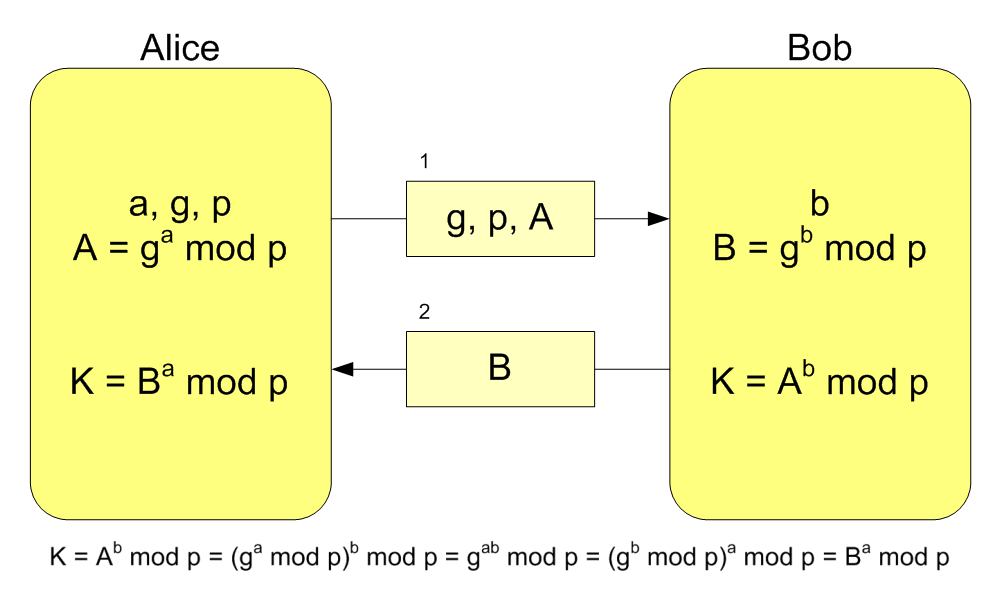
\includegraphics[width=0.6\textwidth]{./figure//D-H}
\caption{Scambio di chiavi Diffie-Hellman, schema di funzionamento.}
\label{FIG:DH}
\end{figure}

\subsubsection{TLS}
Il TLS (Transport Layer Security) � un protocollo crittografico, utilizzato su reti TCP/IP per cifrare delle comunicazioni tra due nodi. Esso viene ampiamente usato per proteggere e-mail, VoIP, web browsing ecc, quindi si occupa di cifrare le connessioni a livello di applicazione del modello ISO/OSI. Al suo interno sono stati implementati vari algoritmi per scambiare le chiavi in maniera sicura e per l'autenticazione come RSA e Diffie-Hellman, AES per la cifratura simmetrica, MD5 e SHA per il controllo dell'integrit� dei dati. Quando due sistemi vogliono comunicare tra loro attraverso TLS devono procedere in tre fasi:

\begin{itemize}
\item handshake e negoziazione tra le parti sugli algoritmi di cifratura da utilizzare (scambio della cipherlist o cipher suite);
\item scambio delle chiavi e autenticazione;
\item scambio di messaggi cifrati in maniera simmetrica e autenticati.
\end{itemize}

\subsubsection{HTTPS}
L'HTTPS (HyperText Transfer Protocol over Secure Socket Layer) � un protocollo per la comunicazione sicura, largamente utilizzato su internet. In pratica HTTPS consiste nella comunicazione tramite il protocollo HTTP all'interno di una connessione criptata da TLS. HTTPS garantisce l'autenticazione del sito web visitato, cifratura dei dati scambiati, protezione della privacy e integrit� dei dati.

\subsubsection{SHA}
SHA (Secure Hash Algorithm) indica una famiglia di cinque algoritmi crittografici, utilizzati per produrre una sorta di impronta digitale del messaggio, chiamato hash. Se indichiamo con $M$ un messaggio qualsiasi e con $\mathcal{H}$ la funzione di hash, allora $D=\mathcal{H}(M)$ sar� diversa per ogni $M'\ne M$. Generalmente algoritmi di questo tipo vengono utilizzati per verificare l'integrit� dei messaggi. Inviando l'hash di un messaggio, insieme al messaggio stesso, il destinatario pu� verificarne l'integrit� ricalcolando la funziona e confrontando il risultato con quello ricevuto dal mittente. Se il messaggio subisce modifiche prima di arrivare a destinazione, l'hash calcolato a destinazione sar� diverso da quello calcolato dalla sorgente.

%Ogni volta che viene scambiato un messaggio, viene anche inviato il suo hash, in modo che il destinatario possa verificare l'integrit� dello stesso ricalcolando la funzione e confrontando il risultato con quello ricevuto.


%diffusi

%\section{Protocolli crittografici}
%HTTPS, TLS, Diffie-Hellman, SHA-1
% ---- ELEMENTI UTILI E GIA' PRONTI! ----
%Secondo capitolo della tesi. Esempio di citazione doppia \cite{Munoz-Lipo,Vas}.

%Esempio di figura in \figurename\ \ref{FIG:LogoUniPD}.
%
%\begin{figure}[!htbp]
%\centering
%
\includegraphics[width=0.25\textwidth]{./figure//LogoUniPD}
%\caption{Esempio di figura.}
%\label{FIG:LogoUniPD}
%\end{figure}
%
%Esempio di tabella in \tablename\ \ref{TAB:Esempio}.
%
%\begin{table}[!htbp]
%\centering
%\renewcommand{\arraystretch}{1.3}
%\caption{Esempio di tabella.}
%\begin{tabular}{cc}
%\hline
%Nome & Valore \\
%\hline
%a & 1 \\
%b & 2 \\
%c & 3 \\
%d & 4 \\
%e & 5 \\
%f & 6 \\
%\hline
%\end{tabular}
%\label{TAB:Esempio}
%\end{table}